\documentclass[a4paper,12pt]{article}
\usepackage{graphicx}
 \usepackage{ragged2e}
\usepackage{geometry}
\usepackage{xcolor}
\usepackage{listings}
\renewcommand{\baselinestretch}{1.5}
\usepackage{mathabx}
\definecolor{mGreen}{rgb}{0,0.6,0}
\definecolor{mGray}{rgb}{0.5,0.5,0.5}
\definecolor{mPurple}{rgb}{0.58,0,0.82}
\definecolor{backgroundColour}{rgb}{0.95,0.95,0.92}
\lstdefinestyle{CStyle}{
    backgroundcolor=\color{backgroundColour},   
    commentstyle=\color{mGreen},
    keywordstyle=\color{magenta},
    numberstyle=\tiny\color{magenta},
    stringstyle=\color{mPurple},
    basicstyle=\footnotesize,
    breakatwhitespace=false,         
    breaklines=true,                 
    captionpos=b,                    
    keepspaces=true,                 
    numbers=left,                    
    numbersep=5pt,                  
    showspaces=false,                
    showstringspaces=false,
    showtabs=false,                  
    tabsize=2,
    language=C
    }
     \lstset{
  backgroundcolor=\color{white}, 
  basicstyle=\footnotesize,        % fonts size
  breaklines=true,                 % line breaking
  captionpos=b,                  
  commentstyle=\color{green},    % comment style
  keywordstyle=\color{blue},       % keyword style
  stringstyle=\color{blue},     % string literal style
}
\usepackage{listings}  
\begin{document}
\begin{center}
\textbf{Assignment-7 \\
\vspace{5mm}
ELP - 718 Telecom Software Laboratory \\
\vspace{2mm}
Pulkit Arora\\
2018JTM2249 \\
2018-2020} \\
\vspace{10mm}
A report presented for the assignment on AWK AND SED\\
\vspace{20mm}

\includegraphics[scale=0.5]{/home/pulkitarora/Downloads/IITD-LOGO.png} \\
\vspace{10mm}
Bharti School Of \\
Telecommunication Technology and Management \\
IIT Delhi \\
India \\
August 16, 2018\\
\tableofcontents
\newpage
\end{center}
%\chapter*{new}
\section{Problem Statement-1}
\subsection{Problem Statement}
{
IT Delhi, has just got the strongest computer. The professors in charge wants to check the computational capacity of the computer. So, they decided to create the problem which is to be given as an assignment to students. Can you help the professor to check the computation capability of the computer?\\
A valid cross is defined here as the two regions (horizontal and vertical) of equal lengths crossing over each other. These lengths must be odd, and the middle cell of its horizontal region must cross the middle cell of its vertical region.
\\
Find the two largest valid crosses that can be drawn on smart cells in the grid, and return two integers denoting the dimension of the each of the two largest valid crosses. In the above diagrams, our largest crosses have dimension of 1,  5 and 9 respectively .\\
\textbf{Note:}The two crosses cannot overlap, and the dimensions of each of the valid crosses should be maximal.\\
The Rate details for the plans opted by the subscribers are -
\subsection{Assumptions}
  \textbf{Constraints}
   \begin{itemize}
   \item 2 <= n <= 105
   \item 2 <= m <= 105
   \end{itemize}

\newpage
\subsection{Screen Shot}
{
\begin{figure}[h]
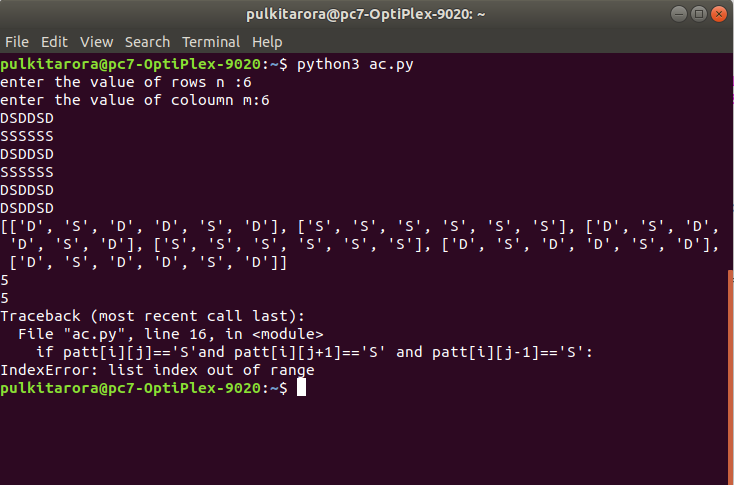
\includegraphics[scale=0.4]{/home/pulkitarora/Pictures/pss1_8.png}
\end{figure}
}
\subsection{INPUT AND OUTPUT FORMAT}
\textbf{INPUT FORMAT}\\
 The first line contains two space-separated integers,  n and m. \\
   Each of the next  lines n contains a string of  m characters where each character is either S (Smart) or D (Dull). These strings represent the rows of the grid. If the jth character in the ith  line is S, then  (i,j) is a  cell smart. Otherwise it's a  dull cell.\\  
\textbf{OUTPUT FORMAT}\\
   Find two valid crosses that can be drawn on smart cell of the grid, and return the dimension of both the crosses in the reverse sorted order(i.e. First Dimension should be the larger one and other should be smaller one).\\
   
   \textbf{Sample Input 0}\\
   5 6\\
SSSSSS\\
SDDDSD\\
SSSSSS\\
SSDDSD\\
SSSSSS\\

\textbf{Sample Output}\\
5 1
\newpage
\section{\large{Problem Statement-2}} 
\subsection{Problem Statement}
\begin{flushleft}
After, getting mix results of valid crosses, professors decided to test the computation abilities on one more problem. This time professors wanted to test the decryption capabilities of the computer.\\
Encryption of  a message requires three keys, k1, k2, and k3. The 26 letters of English and underscore are divided in three groups,  [a-i] form one group, [j-r] a second group, and everything else ([s-z] and underscore) the third group. Within each group the letters are rotated left by ki positions in the message. Each group is rotated independently of the other two. Decrypting the message means doing a right rotation by ki positions within each group.\\
\end{flushleft}
\subsection{INPUT AND OUTPUT FORMAT}
\textbf{INPUT FORMAT}\\
 All input strings comprises of only lowercase English alphabets and underscores(\_).\\
\textbf{OUTPUT FORMAT}\\
 For each encrypted message, the output is a single line containing the decrypted string.\\
   
   \textbf{Sample Input 1}\\
   2 3 4\\
   dikhtkor\_ey\_tec\_ocsusrsw\_ehas\_
   \\
   
   \textbf{Sample Output 1}\\
   hardwork\_is\_the\_key\_to\_success
\subsection{Assumptions}
  \textbf{Constraints}
   \begin{itemize}
   \item 1 <= Length of the string <=150
   \item 1<= ki <=150 (i=1,2,3)
   \end{itemize}

\subsection{Screen Shot}
{
\begin{figure}[h]
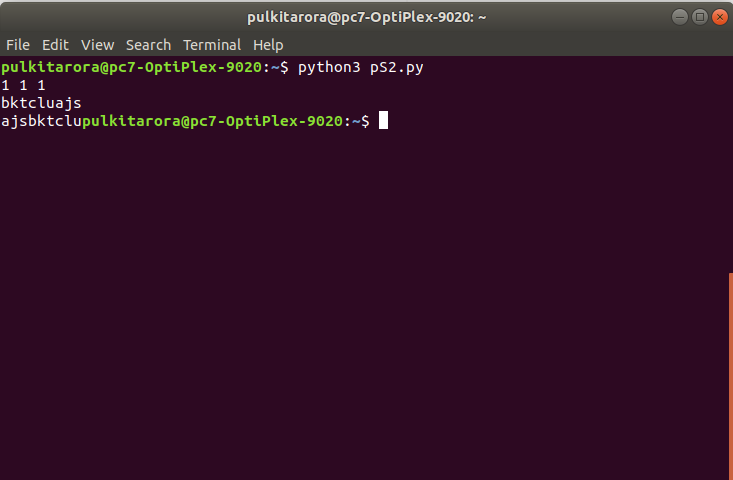
\includegraphics[scale=0.35]{/home/pulkitarora/Pictures/pS2_8.png}
\end{figure}
}
\subsection{Algorithm and Implementation}
 \begin{itemize}
 \item{Create a ps2.awk andoutput.txt file}
 \end{itemize}
\subsection{Code for ps1}
\textbf{ps1.py}
\lstinputlisting[language=C]{/home/pulkitarora/Desktop/assignment-8/ps1.py}
\subsection{Code for ps2}
\textbf{ps2.py}
\lstinputlisting[language=C]{/home/pulkitarora/Desktop/assignment-8/ps2.py}
\nocite{*}
\bibliographystyle{plain}
\bibliography{assign.bib}
\end{document}
